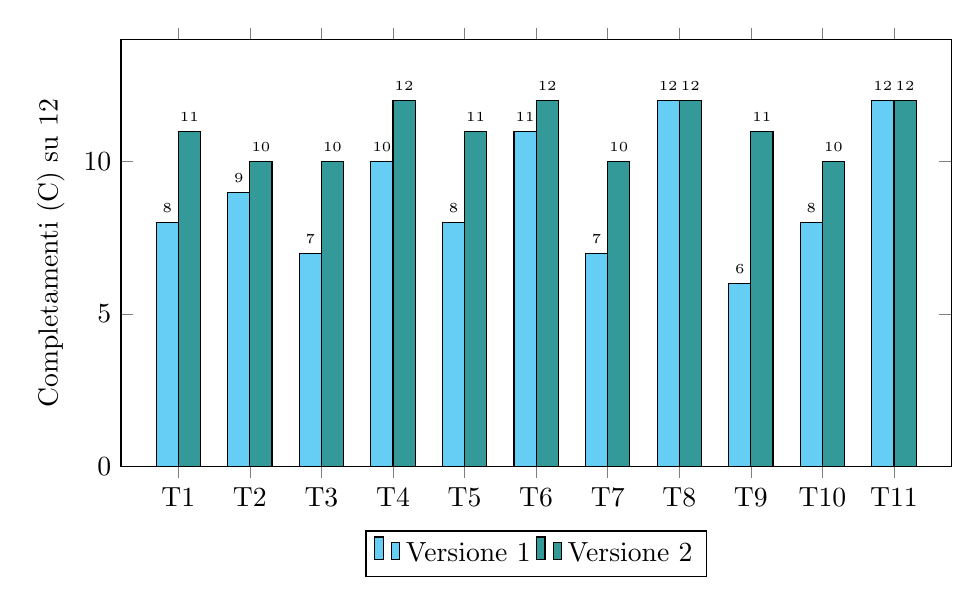
\begin{tikzpicture}
    \begin{axis}[
        ybar=0pt,
        bar width=8pt,
        enlarge x limits=0.08,
        legend style={at={(0.5,-0.15)}, anchor=north, legend columns=-1},
        ylabel={Completamenti (C) su 12},
        symbolic x coords={T1, T2, T3, T4, T5, T6, T7, T8, T9, T10, T11},
        xtick=data,
        nodes near coords,
        nodes near coords align={vertical},
        every node near coord/.append style={font=\tiny},
        width=\textwidth,
        height=7cm,
        ymin=0,
        ymax=14
    ]
        \addplot[fill=cyan!60] coordinates { (T1,8) (T2,9) (T3,7) (T4,10) (T5,8) (T6,11) (T7,7) (T8,12) (T9,6) (T10,8) (T11,12) };
        \addplot[fill=teal!80] coordinates { (T1,11) (T2,10) (T3,10) (T4,12) (T5,11) (T6,12) (T7,10) (T8,12) (T9,11) (T10,10) (T11,12) };
        \legend{Versione 1, Versione 2}
    \end{axis}
\end{tikzpicture}